\begin{figure}
    \centering



\tikzset{every picture/.style={line width=0.75pt}} %set default line width to 0.75pt        

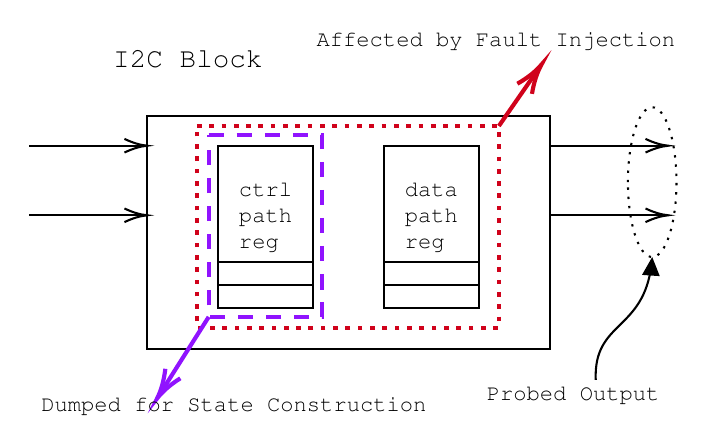
\begin{tikzpicture}[x=0.75pt,y=0.75pt,yscale=-1,xscale=1]
%uncomment if require: \path (0,300); %set diagram left start at 0, and has height of 300

%Shape: Rectangle [id:dp9326819923068139] 
\draw   (397.96,61.38) -- (591.95,61.38) -- (591.95,174) -- (397.96,174) -- cycle ;
%Straight Lines [id:da8579060622058785] 
\draw    (591.95,75.9) -- (647.01,75.9) ;
\draw [shift={(649.01,75.9)}, rotate = 180] [color={rgb, 255:red, 0; green, 0; blue, 0 }  ][line width=0.75]    (10.93,-3.29) .. controls (6.95,-1.4) and (3.31,-0.3) .. (0,0) .. controls (3.31,0.3) and (6.95,1.4) .. (10.93,3.29)   ;
%Straight Lines [id:da837066861655545] 
\draw    (591.95,109.42) -- (647.01,109.42) ;
\draw [shift={(649.01,109.42)}, rotate = 180] [color={rgb, 255:red, 0; green, 0; blue, 0 }  ][line width=0.75]    (10.93,-3.29) .. controls (6.95,-1.4) and (3.31,-0.3) .. (0,0) .. controls (3.31,0.3) and (6.95,1.4) .. (10.93,3.29)   ;
%Straight Lines [id:da0024830437913780923] 
\draw    (395.96,109.42) -- (340.91,109.42) ;
\draw [shift={(397.96,109.42)}, rotate = 180] [color={rgb, 255:red, 0; green, 0; blue, 0 }  ][line width=0.75]    (10.93,-3.29) .. controls (6.95,-1.4) and (3.31,-0.3) .. (0,0) .. controls (3.31,0.3) and (6.95,1.4) .. (10.93,3.29)   ;
%Straight Lines [id:da9595725272918905] 
\draw    (395.96,75.9) -- (367.15,75.9) -- (340.91,75.9) ;
\draw [shift={(397.96,75.9)}, rotate = 180] [color={rgb, 255:red, 0; green, 0; blue, 0 }  ][line width=0.75]    (10.93,-3.29) .. controls (6.95,-1.4) and (3.31,-0.3) .. (0,0) .. controls (3.31,0.3) and (6.95,1.4) .. (10.93,3.29)   ;
%Shape: Rectangle [id:dp3692381690862372] 
\draw   (432.2,75.9) -- (477.84,75.9) -- (477.84,154.11) -- (432.2,154.11) -- cycle ;
%Straight Lines [id:da641212380280751] 
\draw    (432.2,131.77) -- (477.84,131.77) ;
%Straight Lines [id:da016965396748415795] 
\draw    (432.2,142.94) -- (477.84,142.94) ;
%Shape: Rectangle [id:dp6397259288159378] 
\draw   (512.07,75.9) -- (557.72,75.9) -- (557.72,154.11) -- (512.07,154.11) -- cycle ;
%Straight Lines [id:da6619404417007224] 
\draw    (512.07,131.77) -- (557.72,131.77) ;
%Straight Lines [id:da5681218634155383] 
\draw    (512.07,142.94) -- (521.43,142.94) -- (557.72,142.94) ;
%Shape: Rectangle [id:dp700600527249986] 
\draw  [color={rgb, 255:red, 144; green, 19; blue, 254 }  ,draw opacity=1 ][dash pattern={on 5.63pt off 4.5pt}][line width=1.5]  (427.63,70.88) -- (482.4,70.88) -- (482.4,158.36) -- (427.63,158.36) -- cycle ;
%Shape: Rectangle [id:dp07083741234570073] 
\draw  [color={rgb, 255:red, 208; green, 2; blue, 27 }  ,draw opacity=1 ][dash pattern={on 1.69pt off 2.76pt}][line width=1.5]  (421.93,66.41) -- (567.42,66.41) -- (567.42,163.72) -- (421.93,163.72) -- cycle ;
%Straight Lines [id:da7847041731451427] 
\draw [color={rgb, 255:red, 144; green, 19; blue, 254 }  ,draw opacity=1 ][line width=1.5]    (427.63,158.36) -- (404.36,195.15) ;
\draw [shift={(402.75,197.68)}, rotate = 302.32] [color={rgb, 255:red, 144; green, 19; blue, 254 }  ,draw opacity=1 ][line width=1.5]    (14.21,-4.28) .. controls (9.04,-1.82) and (4.3,-0.39) .. (0,0) .. controls (4.3,0.39) and (9.04,1.82) .. (14.21,4.28)   ;
%Straight Lines [id:da28616250433266277] 
\draw [color={rgb, 255:red, 208; green, 2; blue, 27 }  ,draw opacity=1 ][line width=1.5]    (567.42,66.41) -- (586.25,39.27) ;
\draw [shift={(587.96,36.8)}, rotate = 484.75] [color={rgb, 255:red, 208; green, 2; blue, 27 }  ,draw opacity=1 ][line width=1.5]    (14.21,-4.28) .. controls (9.04,-1.82) and (4.3,-0.39) .. (0,0) .. controls (4.3,0.39) and (9.04,1.82) .. (14.21,4.28)   ;
%Shape: Ellipse [id:dp4541297034055598] 
\draw  [dash pattern={on 0.84pt off 2.51pt}] (629.61,93.44) .. controls (629.61,73.51) and (634.84,57.36) .. (641.3,57.36) .. controls (647.76,57.36) and (653,73.51) .. (653,93.44) .. controls (653,113.37) and (647.76,129.53) .. (641.3,129.53) .. controls (634.84,129.53) and (629.61,113.37) .. (629.61,93.44) -- cycle ;
%Curve Lines [id:da48121849953597806] 
\draw    (641.01,132.69) .. controls (637.21,165.58) and (612.98,160.03) .. (614.09,188.74) ;
\draw [shift={(641.3,129.53)}, rotate = 94.03] [fill={rgb, 255:red, 0; green, 0; blue, 0 }  ][line width=0.08]  [draw opacity=0] (8.93,-4.29) -- (0,0) -- (8.93,4.29) -- cycle    ;

% Text Node
\draw (455.02,128.66) node [anchor=south] [inner sep=0.75pt]  [font=\footnotesize] [align=left] {{\fontfamily{pcr}\selectfont ctrl}\\{\fontfamily{pcr}\selectfont path}\\{\fontfamily{pcr}\selectfont reg}};
% Text Node
\draw (534.9,128.66) node [anchor=south] [inner sep=0.75pt]  [font=\footnotesize] [align=left] {{\fontfamily{pcr}\selectfont data}\\{\fontfamily{pcr}\selectfont path}\\{\fontfamily{pcr}\selectfont reg}};
% Text Node
\draw (380.14,28.21) node [anchor=north west][inner sep=0.75pt]   [align=left] {{\fontfamily{pcr}\selectfont I2C Block}};
% Text Node
\draw (345.47,195.16) node [anchor=north west][inner sep=0.75pt]  [font=\footnotesize] [align=left] {{\footnotesize {\fontfamily{pcr}\selectfont Dumped for State Construction}}};
% Text Node
\draw (478.09,19.53) node [anchor=north west][inner sep=0.75pt]  [font=\footnotesize] [align=left] {{\footnotesize {\fontfamily{pcr}\selectfont Affected by Fault Injection}}};
% Text Node
\draw (560.12,190.47) node [anchor=north west][inner sep=0.75pt]  [font=\footnotesize] [align=left] {{\footnotesize {\fontfamily{pcr}\selectfont Probed Output}}};


\end{tikzpicture}
    \caption{scheme of probes placement and affected/dumped registers}
    \label{fig:prob_place}
\end{figure} 
